%!TEX root = main.tex

\section{Motivation}
\label{sec:motivate}

We start with the background on \vr video streaming and the existing approaches.
We then outline the new \vr video-specific opportunities inspired by a deeper understanding of how viewers perceive the quality of \vr videos, and show the potential gains in user-perceived \vr video quality under limited available bandwidth. 
The section ends with a highlight on the key challenges to realize these potential gains.


\subsection{Background of \vr video streaming}
\label{subsec:background}

%\mypara{\vr video streaming}
%\mypara{\vr videos coming to age}
\vr video streaming is coming to age. 
Almost all major content providers (YouTube~\cite{??}, Facebook~\cite{??}, Netflix~\cite{??}, Vimeo~\cite{??}, Amazon Prime~\cite{??}, Hulu~\cite{??}, iQIYI~\cite{??}, YouKu~\cite{??}) launched streaming services for \vr videos across many VR platforms~\cite{oculus,samsung,daydreams,etc}, believing that \vr videos are the future of story telling. 
By 2022, there will be over 55 million active VR headsets in the US, which is as many as paying Netflix members in the US in 2018~\cite{https://qz.com/1298512/vr-could-be-as-big-in-the-us-as-netflix-in-five-years-study-shows/}.
\jc{add more concrete statistics on the popularity of VR}

%\mypara{Delivery architecture} 
Besides the proliferation of the content and devices for \vr videos, the rise of \vr videos is also spurred by its efficient video streaming architecture.
Similar to non-\vr videos, a typical \vr video delivery pipeline is as following. 
A regular video is first encoded using a \vr encoder, and then just as regular videos, the \vr video will be chunked into segments, sent to a content delivery network (CDN) for Internet-scale distribution, and streamed from the CDN edge HTTP servers to \vr headset over the HTTP(S) protocol~\cite{hls,https://www.wowza.com/solutions/streaming-types/virtual-reality-and-360-degree-streaming}.
Like the streaming protocols for non-\vr videos, the \vr-video streaming protocols seek to achieve better {\em QoE-bandwidth tradeoffs}---adapting the quality level (\eg bitrate or quantization parameters) in order to maximize the user-perceived QoE (explained in the next section) under the changing available bandwidth.
\jc{other than the client-side adaptation scheme, is there some fundamental diff or non-trivial steps involved in the preparation/dissemination of \vr content?}


%\mypara{Existing \vr video streaming protocols}
While both the quality adaptation of \vr videos and that of traditional videos share the goal of optimizing the QoE-bandwidth tradeoff, a distinctive feature of \vr video streaming is that the viewer's attention is {\em unevenly} distributed over a large panoramic space with more attention centered around the viewport. 
This is in contrast to non-\vr videos that are displayed on desktop or smartphone screens directly in front of the viewers, making the unevenness of attention less obvious.

Therefore, besides adapting the video quality level along the temporal dimension, \vr streaming protocols also explore the {\em spatial} dimension---each video frame can be spatially partitioned into tiles, and each tile can be streamed and rendered at different quality levels.
This tile-level adaptation enables the protocol to set the quality level of each tile depending on its {\em distance-to-viewport} ({\em DoV}): higher quality around the user's viewport at the cost of areas further from viewport, thus using the same or even less bandwidth. 

%These {\em viewport-driven} protocols (\eg~\cite{??,??,??}) that the user-perceived quality of a spatial region is a function of the encoded quality and the region's distance to the viewport center.
The gain of these {\em DoV-driven} protocols (\eg~\cite{??,??,??}), however, is limited, since the videos have to be encoded with very short chunks so that the quality level can be adjusted whenever the viewport moves substantially. 
We see an increasing interest recently to improve the viewport-driven streaming~\cite{??,??,??} with better viewport prediction algorithms, but the basic limit remains.


\begin{figure}[t!]
  \centering
  \includegraphics[width=0.5\textwidth]{figures/example-velocity.pdf}
  \caption{Illustrative examples of the first \vr video-specific factor. 
  Viewers tend to be insensitive to quality distortions of the objects moving at a high speed relative to the viewport, which can be (a) an object moving across a static viewport, or (b) the viewport moving across a static background. The yellow boxes indicate the viewport. 
  In (a) and (b), the left-hand side and the right-hand side have similar perceived QoE, despite the quality distortions on some objects.}
  \label{fig:example-velocity}
  \end{figure}

\begin{figure}[t!]
  \centering
  \includegraphics[width=0.5\textwidth]{figures/example-luminance-fov.pdf}
  \caption{Illustrative examples of the 2nd and 3rd \vr video-specific factors. 
  Viewers tend to be insensitive to quality distortions when (a) adapting to changes in luminance and when (b) an object has a different field-of-depth to the viewport.
  The dashed boxes and solid boxes indicate where the viewport was and where it is now, respectively.
  In both sub-figures, the left-hand side and the right-hand side have similar perceived QoE, despite the quality distortions on some objects.}
  \label{fig:luminance}
  \end{figure}

\subsection{New \vr video-specific opportunities}
\label{subsec:opportunities}

While the uneven distribution of the viewer's attention affects the QoE-bandwidth tradeoff, our first key observation is that it is just one of {\em several \vr video-specific factors that can heavily influence the perceived QoE of \vr videos but have yet to be fully explored}. 
In particular, this paper examines the three following factors:

\jc{need to visualize the three factors}

\myparashort{Factor\#1: Viewpoint moving speed.} 
One of the most highlighted features of \vr videos is that users can freely move their viewpoints. 
When a viewer moves her viewpoint, her sensitivity to the quality distortion drops in proportional to the speed of the viewport movement.
Consequently, as the viewers watch the video while moving their heads, they sometime report higher perceived quality than other static viewer perceive on the same video at the same objective quality level.
%the perceived quality is significantly improved, since user is unable to detect the distortion. 


\myparashort{Factor\#2: Switches of luminance.} 
As the viewer moves her view around, the viewed region may switch between different levels of brightness, or luminance. 
%When user wears a HMD in VR display, environmental brightness perceived by eyes is totally depended on luminance of video content itself.  
One of our findings is that when the scene changes dramatically from dark to light or vise versa, user's ability of detecting quality distortion also drops for a short period of time (typically \fillme seconds).
As a result, when watching the same content encoded in the same objective quality, people report different levels of subjective quality depending on whether they have just watched something in different levels of luminance.


\myparashort{Factor\#3: Depth of Field (DoF).} \jc{this should be the adaptation of DoF?}
A \vr display can simulate different depths-of-field (DoF) by showing the same object to the eyes with a specific binocular parallax (disparity). 
We found that objects with small DoF (\ie closer to the viewer) have greater parallax, which lowers the viewer's sensitivity to quality distortion due to binocular fusion.
As a result, a viewer might give different levels of attention to the objects of different DoF's, even if they are all close to the center of the viewport.\footnote{This paper assumes the object closest to the center of the viewport is the one watched by the viewer, which may not always hold. But this can be fixed if some gaze tracking mechanism (\eg~\cite{??,??}) is employed.}






\mypara{Prevalence of the \vr video-specific factors}
%According to our data analysis, more than \fillme\% time, user's viewpoint is moving faster than \fillme \textdegree/s. 
One of the most highlighted feature of VR video is that users can freely move their viewpoints. According to our data analysis, more than 30\% viewpoints are moving faster than 20 deg/s. (Fig. \ref{CDFspeed}) 
When human viewpoint is moving, visual acuity is decreased in 2 different conditions: (1) if user is tracking an object, visual acuity decreases smoothly with viewpoint moving speed increases. (2) If user is not tracking an object, visual acuity decreases dramatically with viewpoint moving speed increases. \cite{speed}
\jc{can you visualize such findings, and also show some numbers about the other two factors?}

\begin{figure}
  \centering
  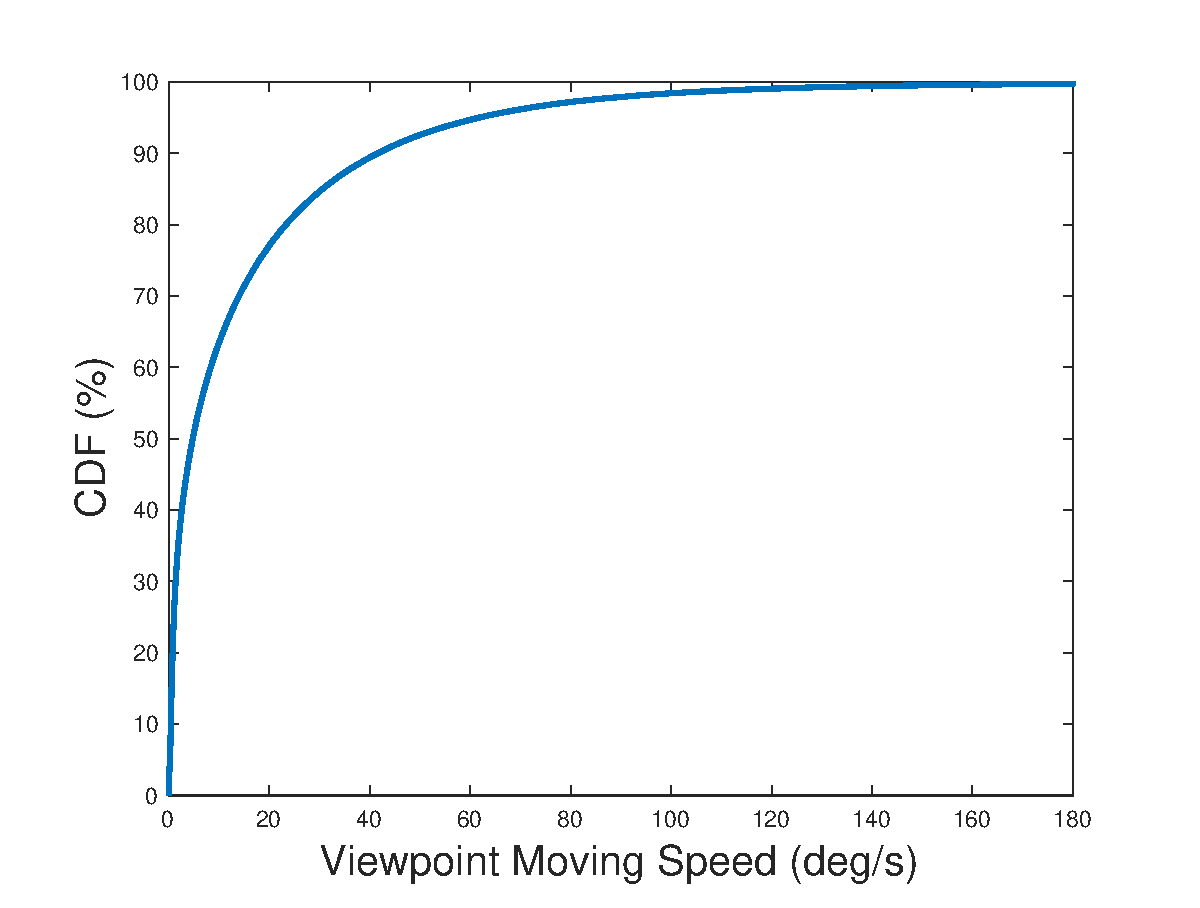
\includegraphics[width=2.5in]{images/speed_CDF.eps}
  \caption{CDF gram of viewpoint moving speed.}
  \label{CDFspeed}
  \end{figure}


%\jc{
%\begin{itemize}
%\item p1: we first extend the jnd model with several \vr specific factors, 1, 2, 3
%\item p2: with the new jnd model (explained latter), the potential improvement is tremendous!
%\end{itemize}
%}


\mypara{Sparser attention leads to less sensitivity}
The intuition behind the new opportunities is that {\em each viewer has a limited span of attention}.
As the video size grows from traditional videos to \vr ones with the new features of panoramic view and immersive experience (\eg DoF), the span of attention, however, does not grow proportionally. 
Consequently, a viewer will give less attention to the specifics of a \vr video, which in turn reduces the sensitivity to quality distortion, creating a multitude of new opportunities, including DoV-driven protocols and the three aforementioned factors, that could lead to better bandwidth-QoE tradeoffs.


%The uneven distribution of \vr user's sensitivities can be explained by the attention theory~\cite{??,??}, which has been successfully applied to specialized video encoder and human-computer interface. 
%The key concept is the just-noticeable difference (JND)---a user tends to notice the difference between two images/videos, only after the difference is greater than a threshold of JND, which depends heavily on the image/video content (as well as the context of the viewer).
%\jc{add a few examples of JND, like content luminance, texture complexity}

%The existing viewport-driven streaming protocols can be seen as one design point of using JND which only depends on the distance between a region and the viewport center. 
%We have seen a few efforts to introduce the existing JND-based attention models in video streaming~\cite{??,??}, although so far their real application so far has been quite limited.


\subsection{Potential for improvement}
\label{subsec:potentials}

Before giving the concrete design of an actual streaming protocol, we first present the potential for improvement of leveraging the \vr-specific factors. 
To do so, we use a metric called PSPNR to denote the perceived quality of a viewer, which can be expressed by $F(P,P',A,v,d,\Delta d,l,\Delta l)$, where $P$ and $P'$ denote the original frame and the rendered frame respectively, $a=(x_a,y_a)$ the viewport center, $v$ the viewport moving speed, $d$ the DoF, $\Delta d$ the change in DoF, $l$ the luminance, and $\Delta l$ the change in luminance. 
We will explain this metric in greater detail in the next section. 
\jc{give a short description of how to understand PSPNR}


We set up a trace-driven experiment to evaluate this potential improvement. PSPNR \cite{PSPNR} is applied as a metric to measure perceived quality. Real traces are collected from over 800 VR displays of 48 users. In our experiment, each video has 5 different bitrate level. We compare the performance of 3 methods:
\begin{itemize}

\item \emph{Viewpoint-driven VR streaming.} Video is cut into 6*12 spatial rectangular tiles. Tiles on user's viewpoint is allocated the high bitrate. For other tiles, bitrate is allocated linearly decreasing with its distance to user's viewpoint.

\item \emph{Perceived quality driven VR streaming. (with 3 VR factors)} Suppose we can freely allocate bitrate to each spatial part of video without video tiling. Besides user viewpoint, content luminance and texture complexity, we also take consideration of viewpoint moving speed, content Depth-of-Field and light / dark adaptation, we do adaptive streaming to maximize user-perceived quality.

\end{itemize}

With consideration of content luminance and texture complexity, perceived-quality-driven VR streaming can save 30\% bandwidth compared with viewpoint-driven VR streaming providing the same PSPNR. Moreover, when we take consideration of viewpoint moving speed, object Depth-of-Field and light / dark adaptation, we can further save 20\% bandwidth.


\begin{figure}
  \centering
  \includegraphics[width=2.5in]{images/improvement.eps}
  \caption{PSPNR-bandwidth tradeoff of (1) Viewpoint-driven VR streaming. (2) Perceived quality driven VR streaming. (3) Perceived quality driven VR streaming. (with 3 VR factors)}
  \label{potential1}
  \end{figure}




\subsection{Key challenges}
In order to achieve perceived quality driven VR streaming, the core challenge is: perceived quality is related to both video content and user behavior, how to take together both-sides information to maximize the perceived quality. For specifically, there are three aspects:

\myparashort{Challenge 1: How to incorporate the unique \vr video-specific factors in the QoE model?}
%Challenge 1: Traditional Human Visual System (HVS) models can not measure perceived quality in VR video display.
Perceived quality can be well-measured in traditional video display by building mathematical model from luminance, texture complexity and viewpoint-object distance to perceived quality. However, as we have mentioned, besides these existing factors, perceived quality in VR display is related to several new factors which are never modeled before. Their mathematical relationship to perceived quality, and how these new factors combined with existing factors together influence perceived quality are unknown problems.

\myparashort{Challenge 2: How to improve coding efficiency by fully exploiting the \vr video-specific opportunities?}
%Challenge 2: Traditional grid-like video tiling scheme performs poorly in perceived quality optimization.
To optimize perceived quality, we need to independently allocate bitrate of each spatial part of the video. Grid-like tiling scheme is a widely used method to solve the problem. Video is cut into several rectangular tiles with equal size which can be independently encoded / decoded. So we can allocate different bitrate to different tiles.

However, traditional grid-like tiling performs poorly in perceived quality optimization in two aspects: 

(1) Coarse-grained tiling causes coarse-grained rate allocation, and perceived quality obtained by coarse-grained rate allocation is far from that obtained by fine-grained rate allocation. We encode the video with different rate allocation granularity. We apply PSPNR to measure perceived quality and Fig. \ref{optimalencoding} shows the PSPNR-bandwidth tradeoff. Rate allocation with 3*6 / 6*12 granularity obtains -x\% / -x\% PSPNR compared with 12*24 granularity, this is a significant performance gap in perceived quality optimization.

\begin{figure}
  \centering
  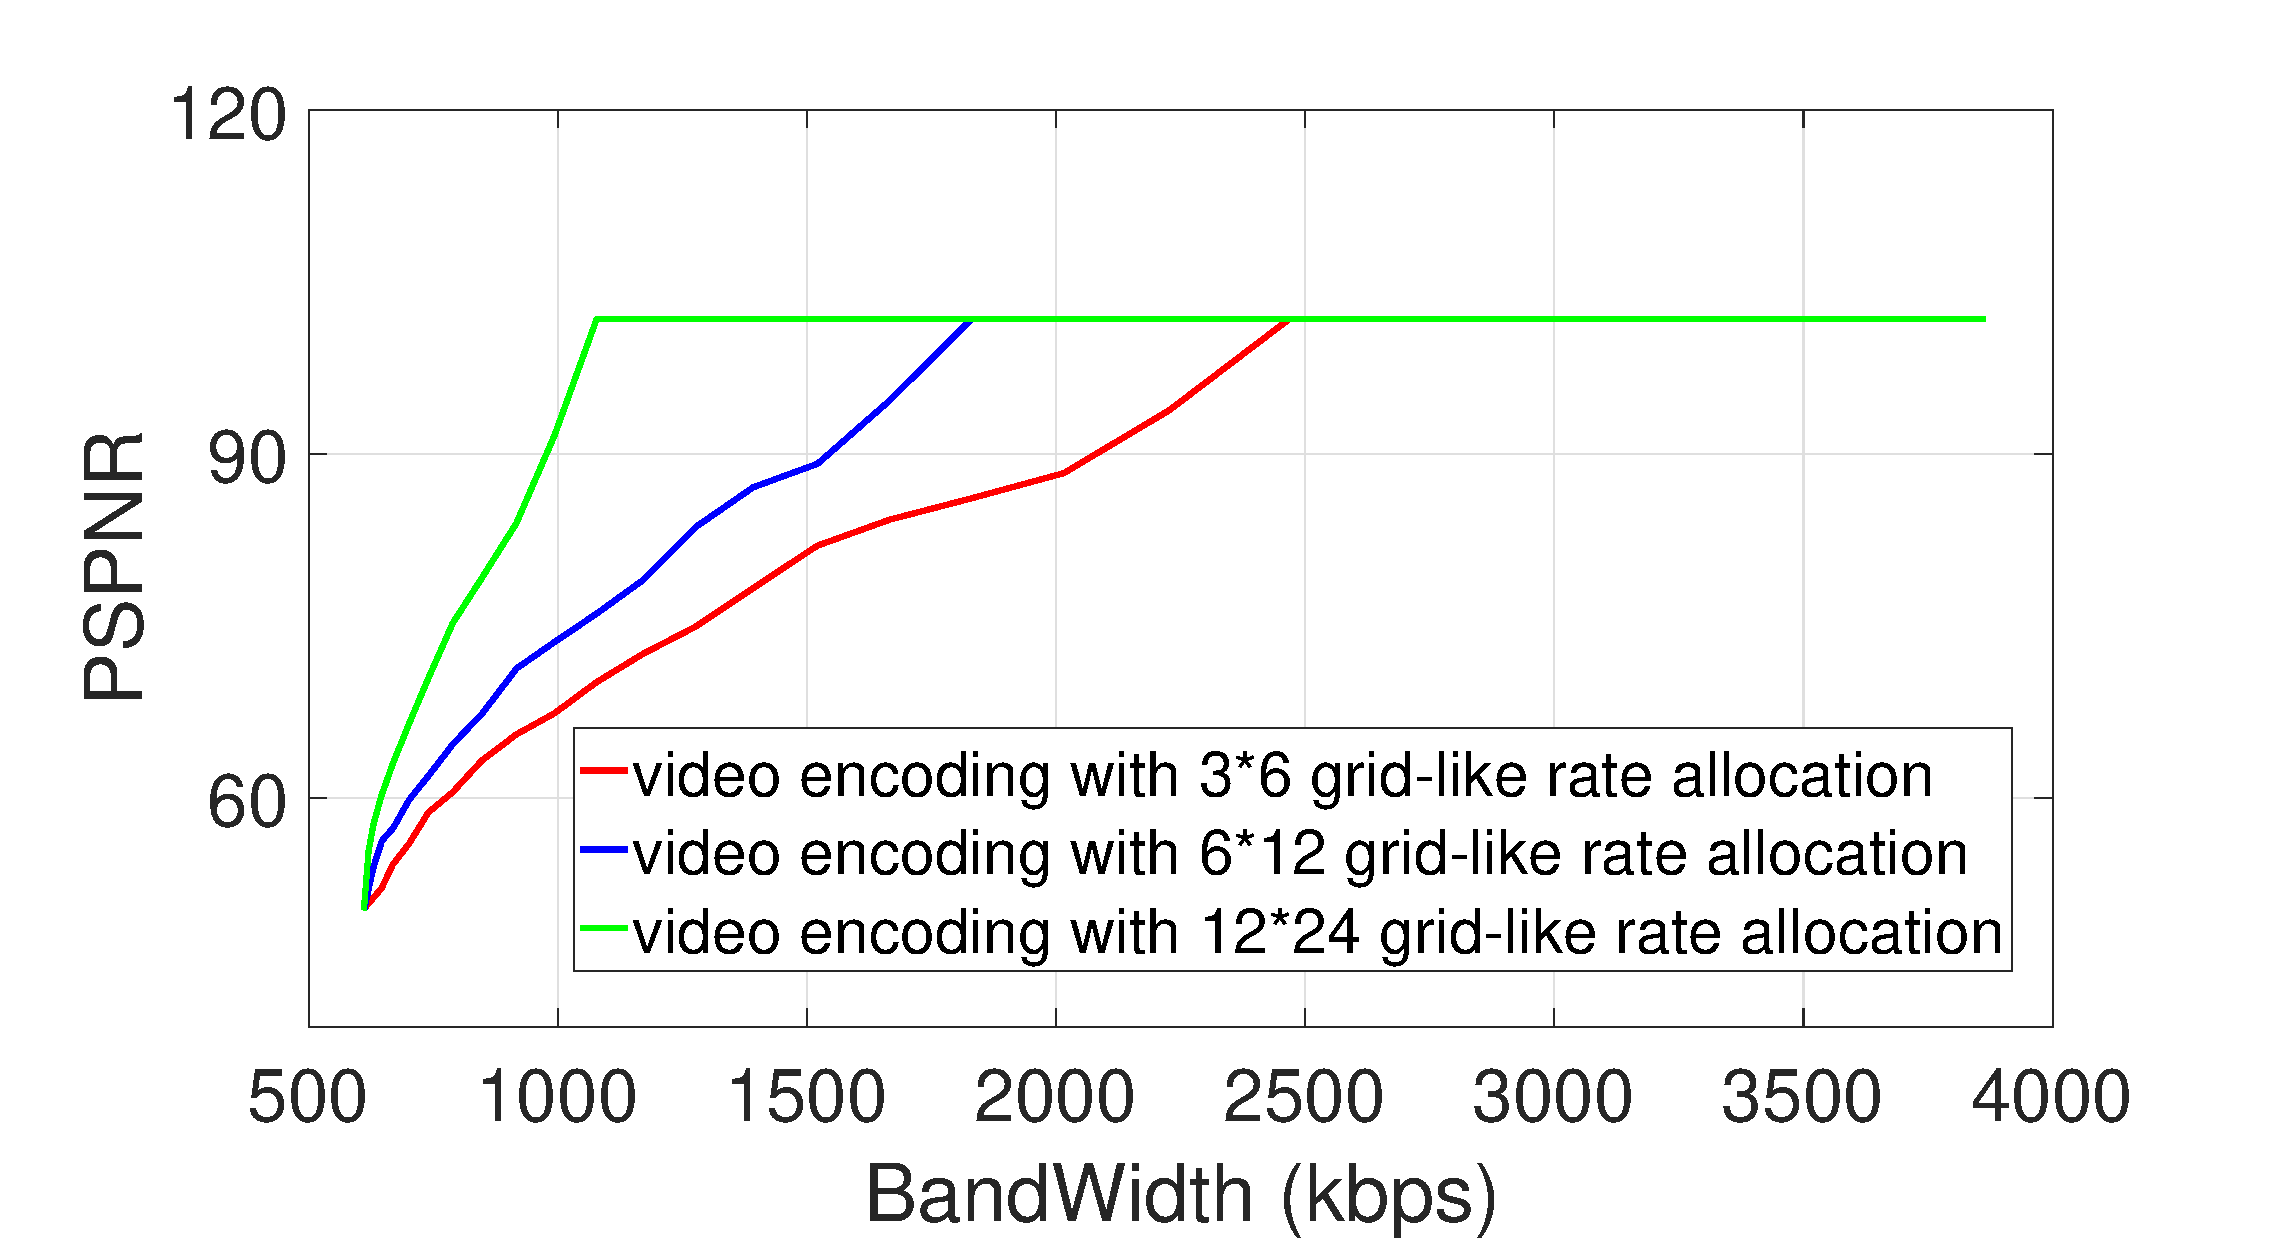
\includegraphics[width=2.5in]{images/optimalencoding.eps}
  \caption{PSPNR-bandwidth tradeoff in video encoding with different granularity of rate allocation.}
  \label{optimalencoding}
  \end{figure}

(2) Fine-grained tiling introduces serious bitrate efficiency problem in video encoding. In practice, each tile has to be encoded independently instead of encoded together. When we cut the video into tiles, the total video size is increased. Fig. \ref{bitrateefficiency} shows the video size of different tiling granularity compared with original video size. We find that cutting a video into 12*24 tiles introduces 50\% to 330\% additional video size compared to original video. This significantly lower its practical performance in perceived quality optimization, especially in low bandwidth situations where the bitrate efficiency problem is very serious.

\begin{figure}
  \centering
  \includegraphics[width=2.5in]{images/bitrateefficiency.eps}
  \caption{The ratio of video size after tiling and original video size in each tiling granularity and each bitrate level. We notice that fine-grained tiling introduces serious bitrate efficiency problem, especially in low bandwidth situations in which the overall bitrate of each tile is low.}
  \label{bitrateefficiency}
  \end{figure}

\myparashort{Challenge 3: How to adapt video quality over existing HTTP-based protocol while the \vr video encoding requires real-time viewer actions as input?}
%Challenge 3: Information needed for perceived quality computation is disparted on server-side and client-side.
To optimize perceived quality, client needs to compute the perceived quality of each bitrate allocation and then make decision. However, different from video quality which only related to video content itself, perceived quality depends on both video content and user behavior. Information of video content is located on server-side while information of user behavior is located on client-side. To get information of video content with current DASH, client has to pre-request in information of each pixel from server. This communication overload even exceed the overload of actual video streaming.



